\section{Method}

\begin{figure}[t!]
    \centering
    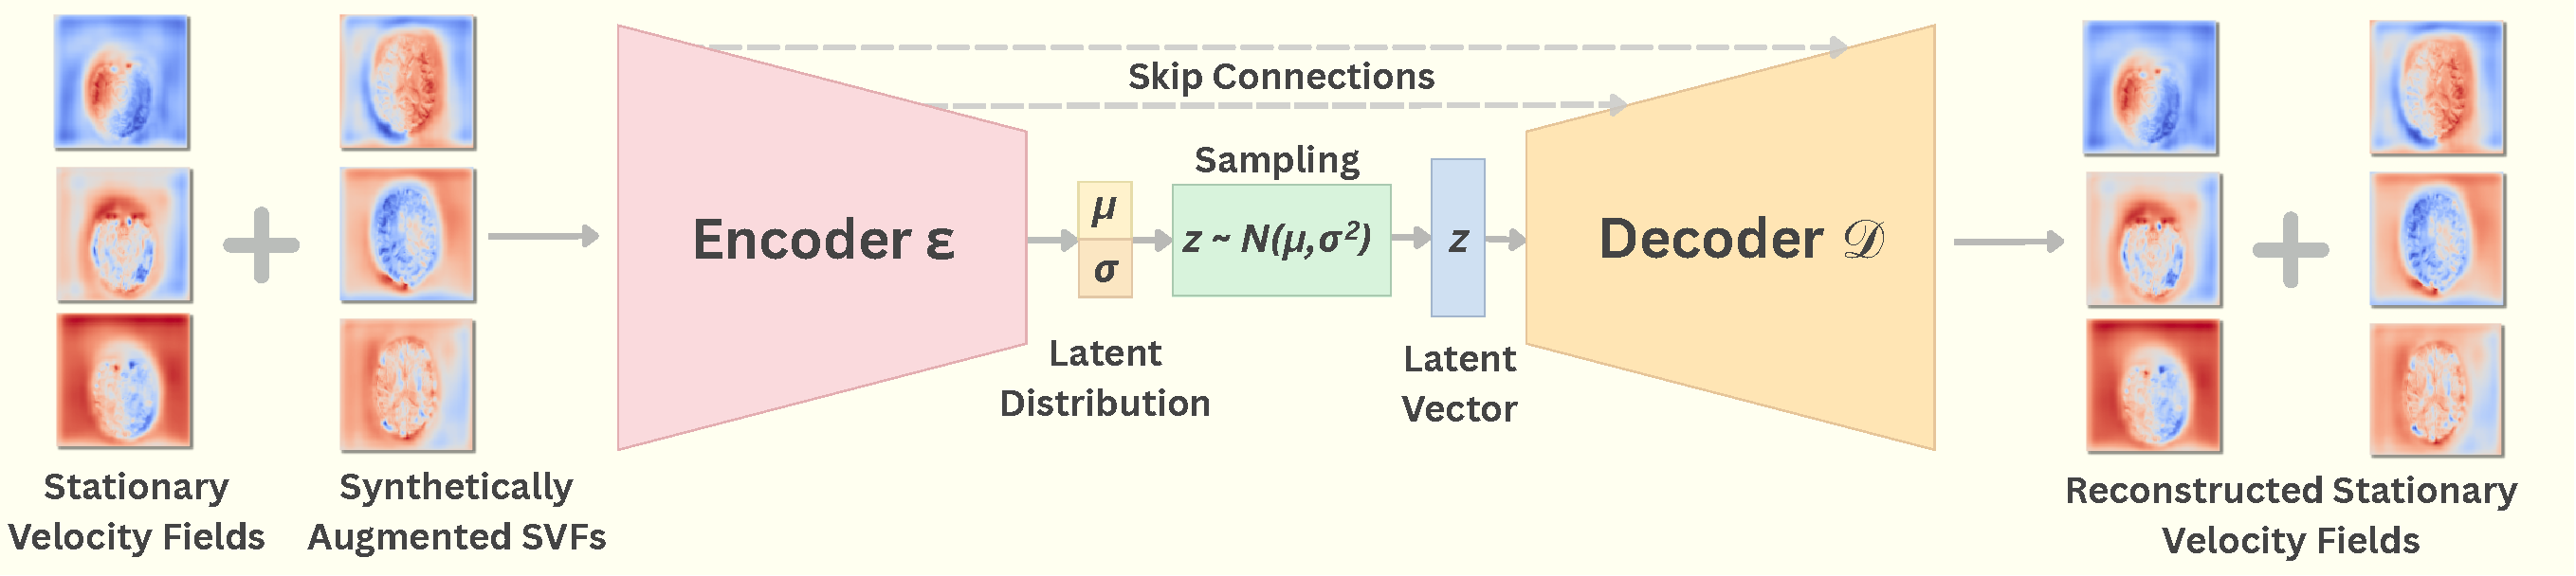
\includegraphics[width=1.0\linewidth]{images/vae-cropped.pdf}
    \caption{Pretraining the 3D variational autoencoder to learn a compact latent representation of baseline-referenced stationary velocity fields (SVFs).}
    \label{fig:vae}
\end{figure}

\begin{figure*}[t!]
    \centering
    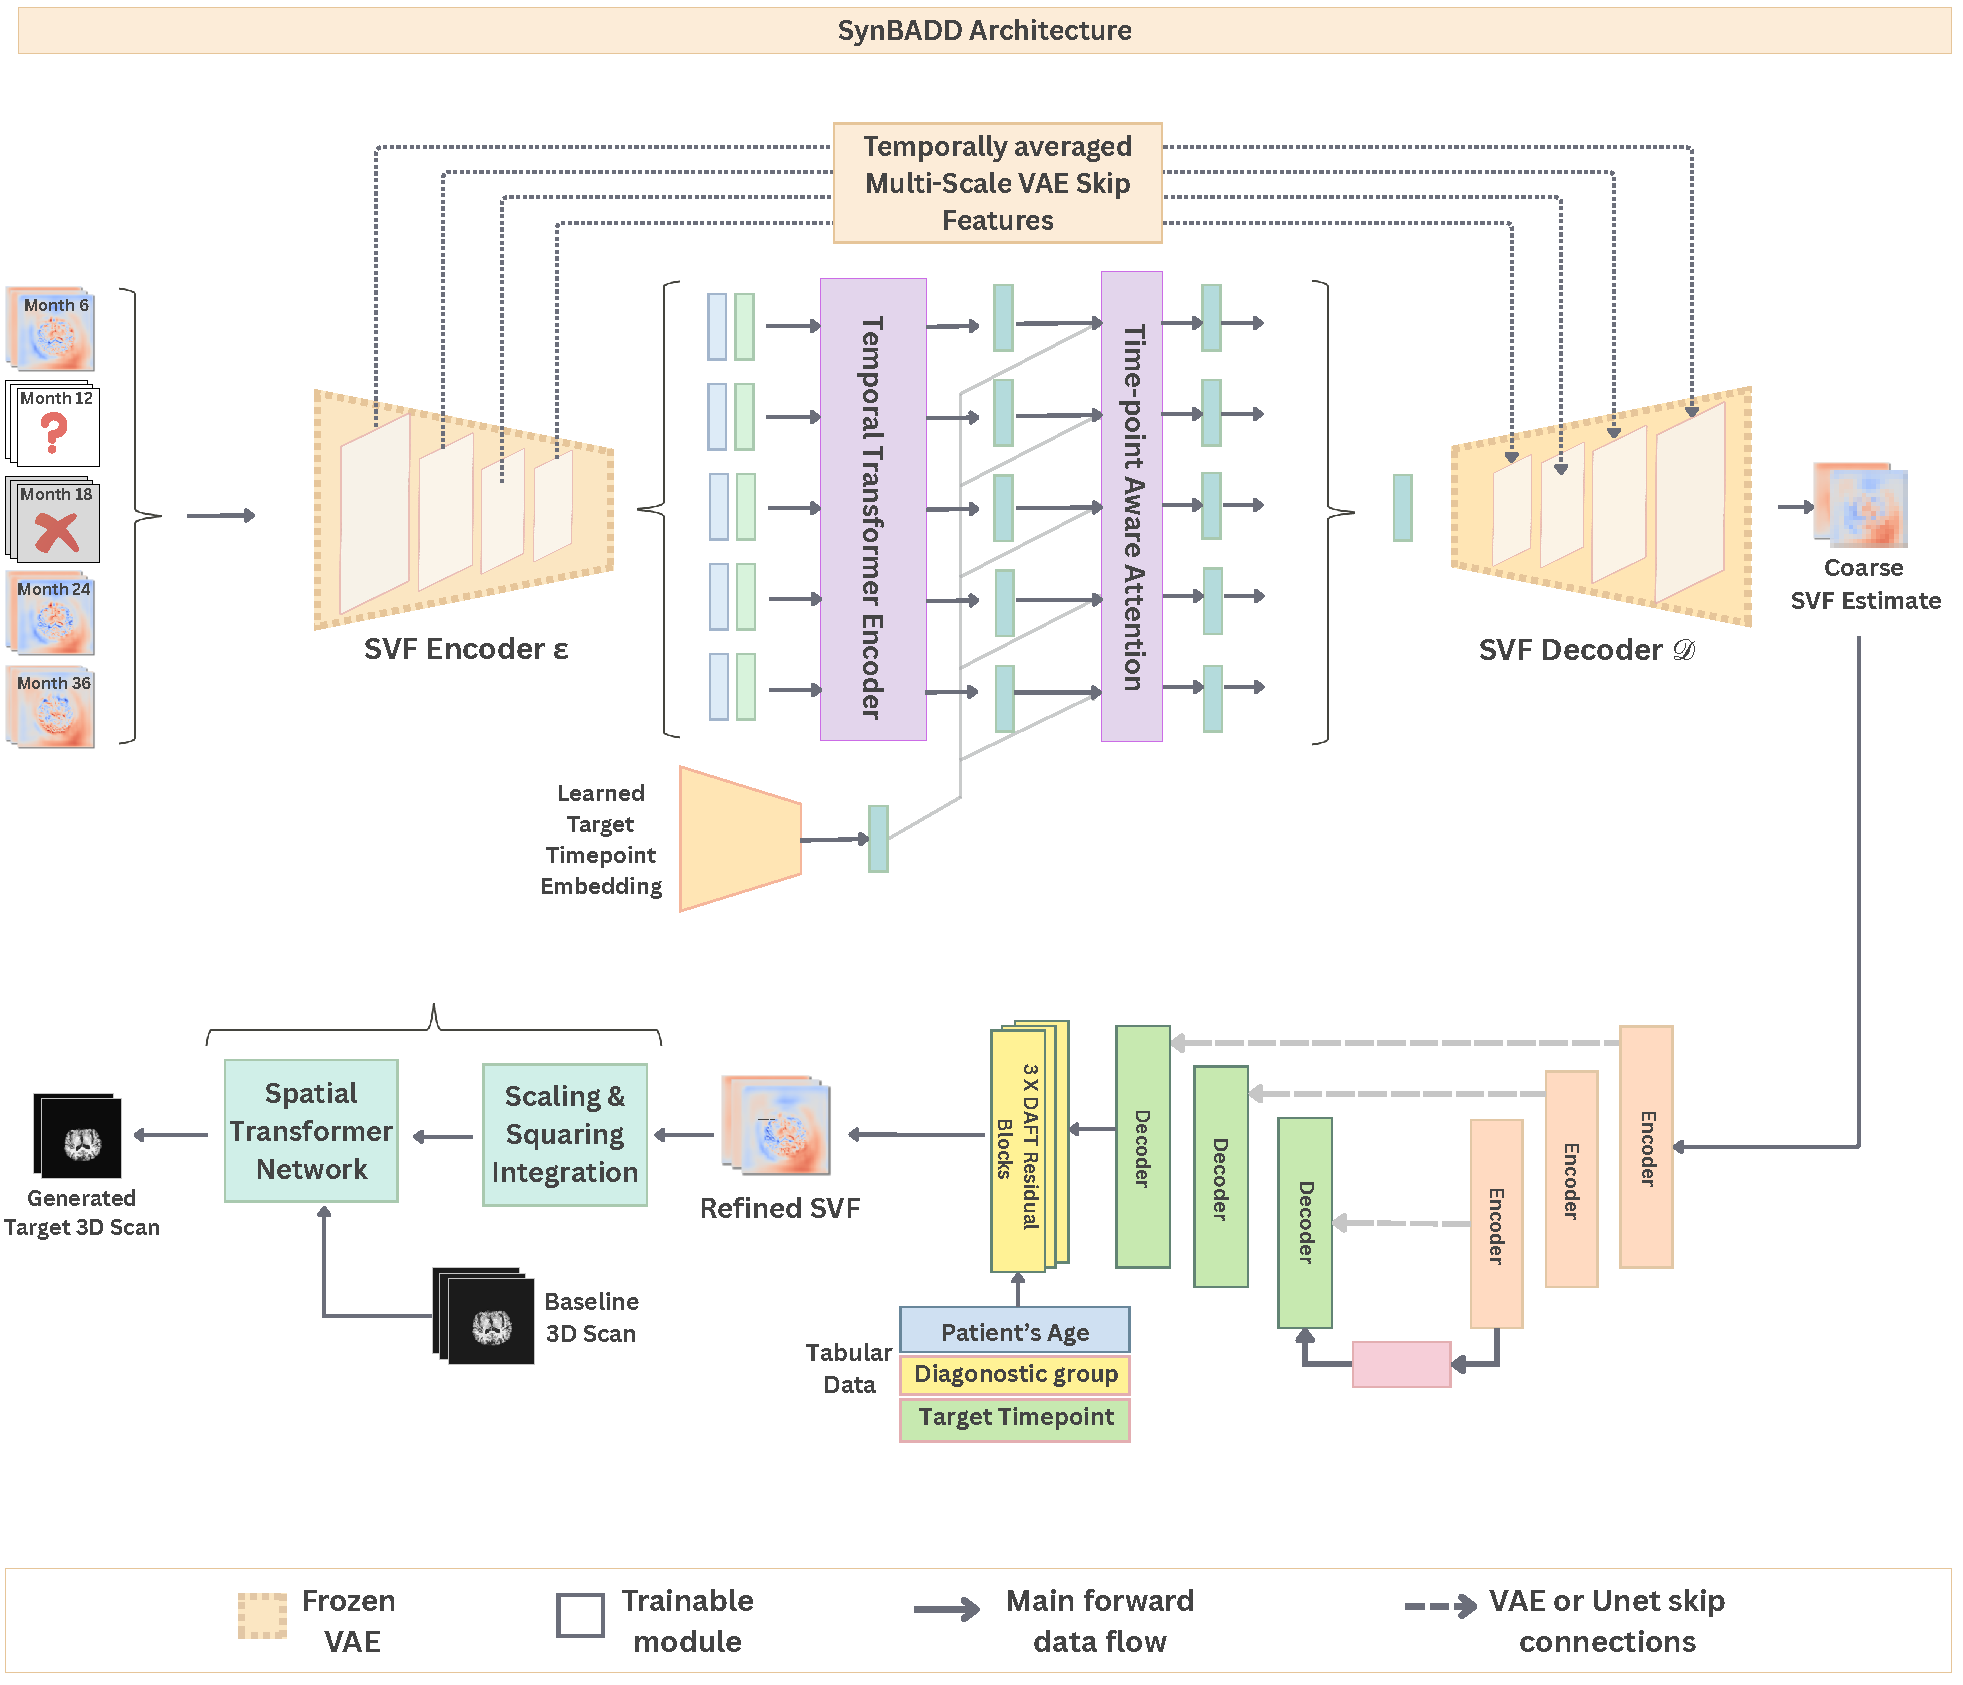
\includegraphics[width=1.0\linewidth]{images/SYNBADD-Main-Architecture.pdf}
    \caption{Overview of SynBADD. A frozen VAE encodes baseline-referenced longitudinal SVFs; a target-aware cross-attention transformer predicts the latent representation at the requested visit; the frozen VAE decoder produces a coarse SVF using temporally averaged multiscale skip features; and a DAFT-conditioned 3D U-Net refines, integrates, and applies the SVF to the screening baseline.}
    \label{fig:overview}
\end{figure*}

We address synthesis of a missing brain MRI at an intermediate point in a longitudinal sequence. Let $I_0$ denote the screening baseline and let $I_{T_i}$ denote a follow-up acquired at one of five scheduled visits, $T_i\in\{\mathrm{m06},\mathrm{m12},\mathrm{m18},\mathrm{m24},\mathrm{m36}\}$. After rigid inter-scan coregistration with ANTs~\cite{avants2008ants}, VoxelMorph registration~\cite{balakrishnan2019voxelmorph,dalca2018unsupervised} provides a baseline-referenced stationary velocity field (SVF) $v_i$ for each observed follow-up. For a held-out target visit $T_p$, SynBADD predicts $\hat v_p$, integrates it to a diffeomorphic displacement $u_p=\exp(\hat v_p)$, and synthesizes
\begin{equation}
    \hat I_{T_p}=I_0\circ(\operatorname{Id}+u_p).
\end{equation}
The framework therefore models longitudinal change in deformation space while retaining the subject's screening scan as the intensity source. As illustrated in Figure~\ref{fig:overview}, it consists of a frozen SVF VAE, a target-aware cross-attention transformer, and a DAFT-conditioned spatial refinement network.

\subsection{Latent Representation Learning of SVFs}

We use a pretrained 3D VAE with U-Net skip connections to represent each three-channel SVF. Its six encoder stages have channel widths $32,64,128,256,512,$ and $512$, with 3D batch normalization and ReLU activations. The encoder produces a 512-dimensional posterior mean $\mu_i$, log-variance $\log\sigma_i^2$, and five multiscale skip tensors $s_i^{(r)}$:
\begin{equation}
    \mu_i,\log\sigma_i^2,\{s_i^{(r)}\}_{r=1}^{5}=\mathcal{E}(v_i).
\end{equation}
During temporal-model training and inference, the VAE is frozen and its deterministic posterior mean $z_i=\mu_i$ is used rather than a sampled latent.

The five follow-up slots are retained in a fixed order. The target slot and any unavailable visit are zero-filled before VAE encoding. At each resolution, the implementation takes an unmasked temporal mean of the resulting skip tensors:
\begin{equation}
    \bar s^{(r)}=\frac{1}{5}\sum_{i=1}^{5}s_i^{(r)}.
\end{equation}
Thus, both observed and zero-filled slots contribute to the decoder's multiscale spatial prior exactly as implemented. The VAE was pretrained separately using SVF reconstruction and latent regularization, with endpoint and angular terms encouraging vector-field fidelity; it remains fixed throughout the main SynBADD optimization.

\subsection{Trajectory Inference via Target-Aware Cross-Attention}

The main temporal model is the base \texttt{CrossAttentionTransformer}. Each of the five latent slots receives a learned positional embedding $e_i^{\mathrm{pos}}$,
\begin{equation}
    x_i=z_i+e_i^{\mathrm{pos}},
\end{equation}
and the resulting sequence is processed by a two-layer, eight-head transformer encoder:
\begin{equation}
    H=\operatorname{TransformerEncoder}(x_1,\ldots,x_5)
    \in\mathbb{R}^{5\times512}.
\end{equation}
The requested target-slot index $p$ addresses a learned embedding table to obtain the single query $q_p\in\mathbb{R}^{512}$. Target-aware dot-product attention then pools the encoded tokens:
\begin{equation}
    \alpha_i=\frac{\exp(q_p^\top H_i)}{\sum_{j=1}^{5}\exp(q_p^\top H_j)},
    \qquad
    \hat z_p=\sum_{i=1}^{5}\alpha_iH_i.
\end{equation}
This final cross-attention operation is single-query dot-product pooling, not an additional multi-head attention block and not the gated-attention variant evaluated in the ablation study. Consistent with the implementation, no explicit padding mask is passed to either the transformer encoder or the final pooling operation; zero-filled slots remain addressable tokens.

\subsection{Image Synthesis with Diffeomorphic Warping}

The frozen VAE decoder combines $\hat z_p$ with the temporally averaged skip hierarchy to obtain a coarse SVF:
\begin{equation}
    \tilde v_p=\mathcal{D}(\hat z_p,\{\bar s^{(r)}\}_{r=1}^{5}).
\end{equation}
The refinement network is a 3D U-Net with encoder widths $(16,32,32,32,32)$ and a skip-connected decoder. DAFT is \emph{not} applied at every encoder or decoder level. It is confined to the final full-resolution refinement stage after the main encoder--decoder path: three consecutive post-decoder blocks modulate feature maps of 35, 32, and 16 channels before convolution. Each DAFT block globally pools its incoming feature map, concatenates the pooled features with the raw three-scalar condition
\begin{equation}
    c=[\text{diagnostic group},\text{age},\text{target-visit index}],
\end{equation}
and predicts channel-wise affine scale and shift parameters. A final $3\times3\times3$ convolution maps the 16-channel representation to the refined three-channel SVF $\hat v_p$.

Scaling-and-squaring integration with ten steps at the full $128^3$ resolution produces $u_p=\exp(\hat v_p)$, after which a differentiable spatial transformer~\cite{jaderberg2015spatial} warps the screening baseline:
\begin{equation}
    \hat I_{T_p}=\operatorname{STN}(I_0,u_p).
\end{equation}
Although the source tensor is named \texttt{latest\_scan} in the implementation, the dataset always loads the screening visit; the synthesis source is therefore the baseline, not the latest available follow-up.

\subsection{Training Objectives}
\label{sec:training_objectives}

Training is separated into VAE pretraining and main-model optimization. In the latter, VAE parameters and encoded features are frozen, while the temporal transformer and refinement generator are optimized jointly.

\subsubsection*{VAE pretraining}

The VAE objective combines voxelwise SVF reconstruction, Kullback--Leibler regularization, endpoint error, and angular error:
\begin{equation}
    \mathcal{L}_{\mathrm{VAE}}=
    \lambda_{\mathrm{recon}}\mathcal{L}_{\mathrm{recon}}+
    \lambda_{\mathrm{KL}}\mathcal{L}_{\mathrm{KL}}+
    \lambda_{\mathrm{EPE}}\mathcal{L}_{\mathrm{EPE}}+
    \lambda_{\mathrm{ang}}\mathcal{L}_{\mathrm{ang}}.
\end{equation}
For velocity vectors $v(x)$ and $\hat v(x)$, endpoint error measures magnitude discrepancy,
\begin{equation}
    \mathcal{L}_{\mathrm{EPE}}=\frac{1}{|\Omega|}
    \sum_{x\in\Omega}\|\hat v(x)-v(x)\|_2,
\end{equation}
while angular error penalizes directional disagreement:
\begin{equation}
    \mathcal{L}_{\mathrm{ang}}=\frac{1}{|\Omega|}\sum_{x\in\Omega}
    \arccos\!\left(
    \frac{\hat v(x)\cdot v(x)}{\|\hat v(x)\|_2\|v(x)\|_2+\epsilon}
    \right).
\end{equation}

\subsubsection*{Main-model optimization}

The main model uses the coefficients in the released configuration:
\begin{equation}
\begin{split}
    \mathcal{L}_{\mathrm{main}}={}&0.2\mathcal{L}_{\mathrm{SSIM}}
    +0.5\mathcal{L}_{\mathrm{VXM}}
    +0.1\mathcal{L}_{\mathrm{fold}}\\
    &+0.05\mathcal{L}_{\mathrm{vol}}
    +0.05\mathcal{L}_{\mathrm{smooth}}.
\end{split}
\end{equation}
Here $\mathcal{L}_{\mathrm{SSIM}}=1-\operatorname{SSIM}(\hat I_{T_p},I_{T_p})$. The VoxelMorph-based term $\mathcal{L}_{\mathrm{VXM}}$ registers the generated and target scans with a frozen pretrained VoxelMorph network and combines three-scale intensity MSE with a small Jacobian-to-unity penalty. It provides deformation-aware image supervision inspired by diffeomorphic registration~\cite{beg2005lddmm,dalca2018unsupervised}.

Let $J(x)$ denote the Jacobian determinant computed after integrating the refined SVF. The two Jacobian penalties are
\begin{equation}
    \mathcal{L}_{\mathrm{fold}}=\operatorname{mean}_{J(x)<0}|J(x)|,
    \qquad
    \mathcal{L}_{\mathrm{vol}}=\operatorname{mean}_{x}|J(x)-1|.
\end{equation}
The first penalizes topology-violating folds, the second discourages extreme local volume change, and $\mathcal{L}_{\mathrm{smooth}}$ is an $L_2$ finite-difference penalty on the refined SVF. The main configuration does not include a separate voxelwise image MSE term, does not impose a Jacobian target of 0.9, and assigns zero weight to direct SVF endpoint and angular losses. The discriminator is disabled, so its configured regularizer is inactive.
